\subsection{Performance of gain and noiserates by temperature variation}
Since signals of Silicon Photomultipliers are very sensible to temperature changes, there is an advantage of studying the gain and noiserate depending on the device temperature. Actually the signal depending on gain should stand the same while running data taking phases. Therefore the bias voltage supplied to the SiPM have to be adjusted under temperature changes. For this reason producers for SiPMs like Hamamatsu whose products we use for our prototyps give a temperature regression coefficient which have to be validated. For our prototyp we also check alternative methods to keep the gain constant due to the fact that measurements of temperature are not very precisely nor it is not checkable if it is the real temperature of the semiconductor.

\subsubsection{Testsetup}
To measure the performance under temperature variation a setup was built up including a cooling box, which was used in the testphase of the silicion strip modules here in aachen.
A version of our frontend board with an higher amplification factor was make use of which could be controled with an external power supply, given the bias voltage to the SiPM. For the measurement of gain and noiserate the outcoming signal was splitted over a Fan-Out and routed to a FADC and a scaler.
The FADC triggers itselves on every flank over $0.5\,\mathrm{p.e.}$. The given pulses then were analysed online and the peakheights were filled into an histogram producing a so called fingerspectrum.
Afterwards the first three p.e.-peaks were fitted by gaussian function and a combination of them were taking as the gain factor which is defined as the distance between two p.e.-peaks.
The line to the scaler were taking to measure the noiserate by connecting a LTD in front of the scaler which discriminates signals over $0.5\,\mathrm{p.e}$.
In total there were three measurement methods to check the changement of the parameter. This three listed in following were done with two several series of SiPMs, S10362-33-050C and S12572-050C.
A sketch of the setup is shown in figure \ref{NoRa_DAQ}. 
\begin{figure}[h]
	\centering
	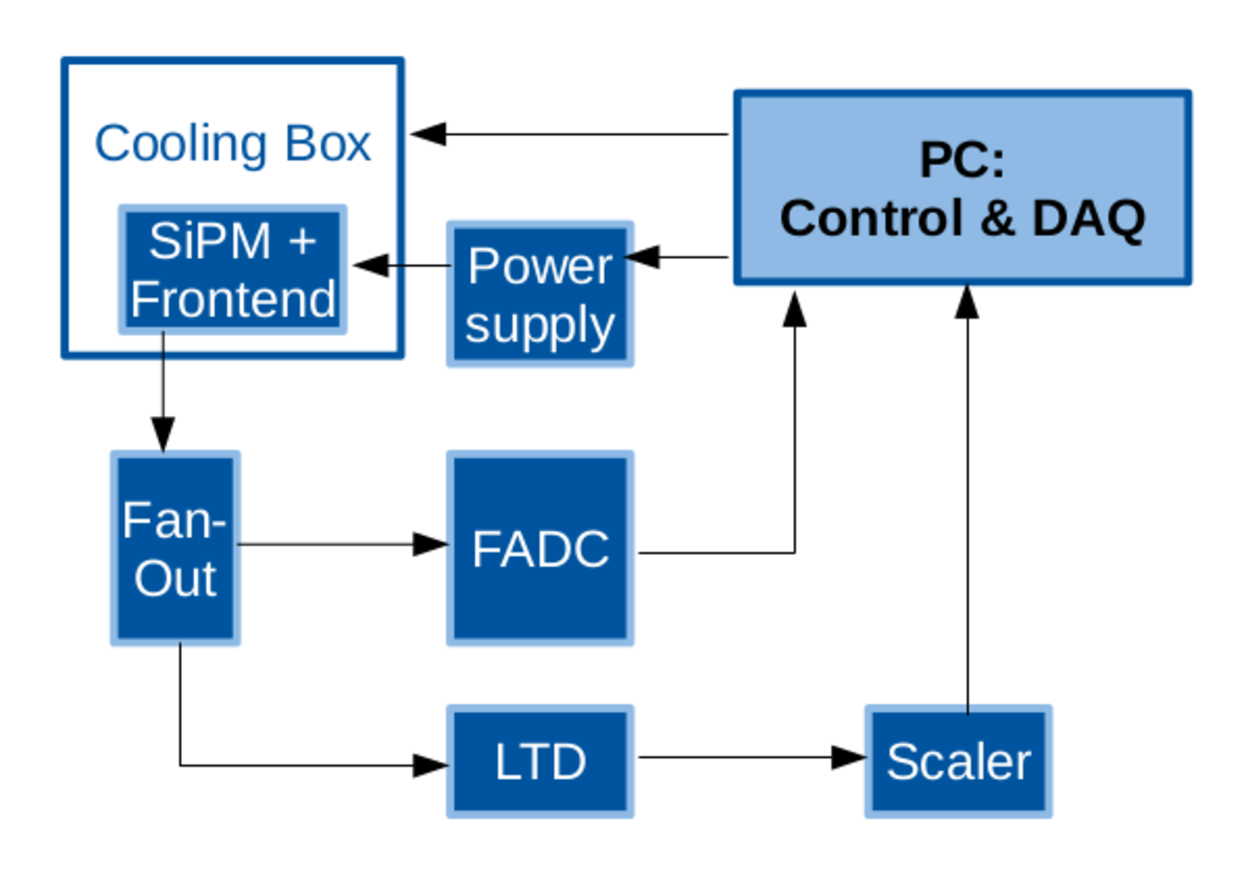
\includegraphics[width = 0.5\textwidth]{Figures/radermacher/NoRa_DAQ_en.pdf}
	\caption{DAQ-Chain for measurements with SiPMs under temperature variation}
	\label{NoRa_DAQ}
\end{figure}
\begin{description}
	\item[Measurement of noiserates by constant gain]: For this method the gain was checked every temperature step and the bias voltage were corrected until the gain was the default value. Afterwards the noiserate were measured over the LTD with a threshold on $0.5\,\mathrm{p.e.}$. With this measurement method it was also possible to check the temperature coefficient.
	\item[Measurement of noiserates and gain by constant bias voltage]: In this measurement simply the bias voltage was fixed to a certain value and every step of temperature the gain and the noiserate was measured.
	\item[Measurement of noiserates and gain by constant temperature]: Here the temperature was fixed and the bias voltage were raised in little steps. 
\end{description}

\subsubsection{spectra analysis}
The spectra one get from this measurements are shown in figure \ref{fingerspecs}. As one can see, there are some differences between the two tested SiPMs. The spectrum of the older version S10362-33-050C shows nearly overlapping p.e. peaks which could not seperated very clearly. Otherwise the noise spectrum only has up to $3\,\mathrm{p.e.}$. The S12572-050C series in contrast shows more than $5\,\mathrm{p.e.}$. On the other hand the p.e.-peaks are clearly seperated which leads to a better gain determination.
\begin{figure}[h]
	\centering
	\begin{minipage}[b]{0.49\textwidth}
		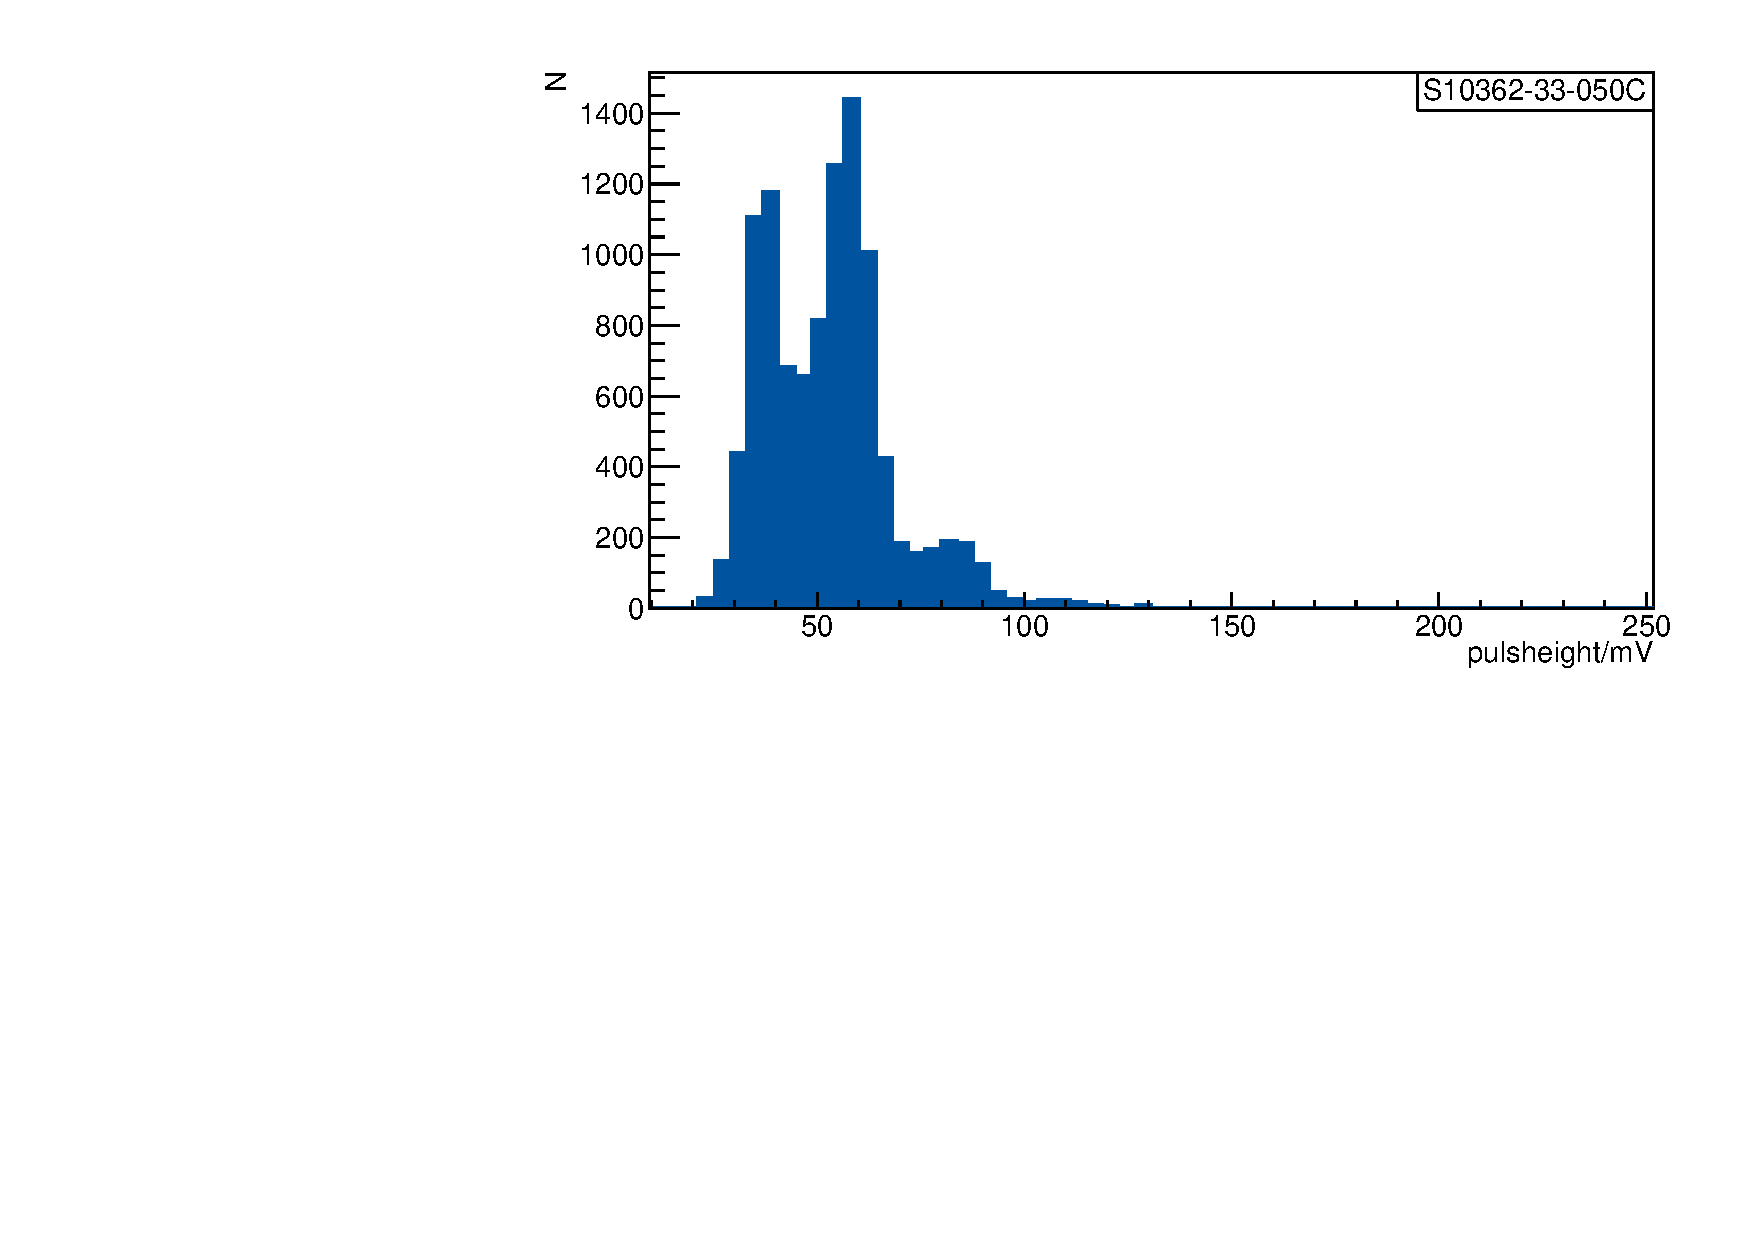
\includegraphics[width = .99\textwidth]{Figures/radermacher/S10362-33-050C.pdf}
	\end{minipage}
	\begin{minipage}[b]{0.49\textwidth}
		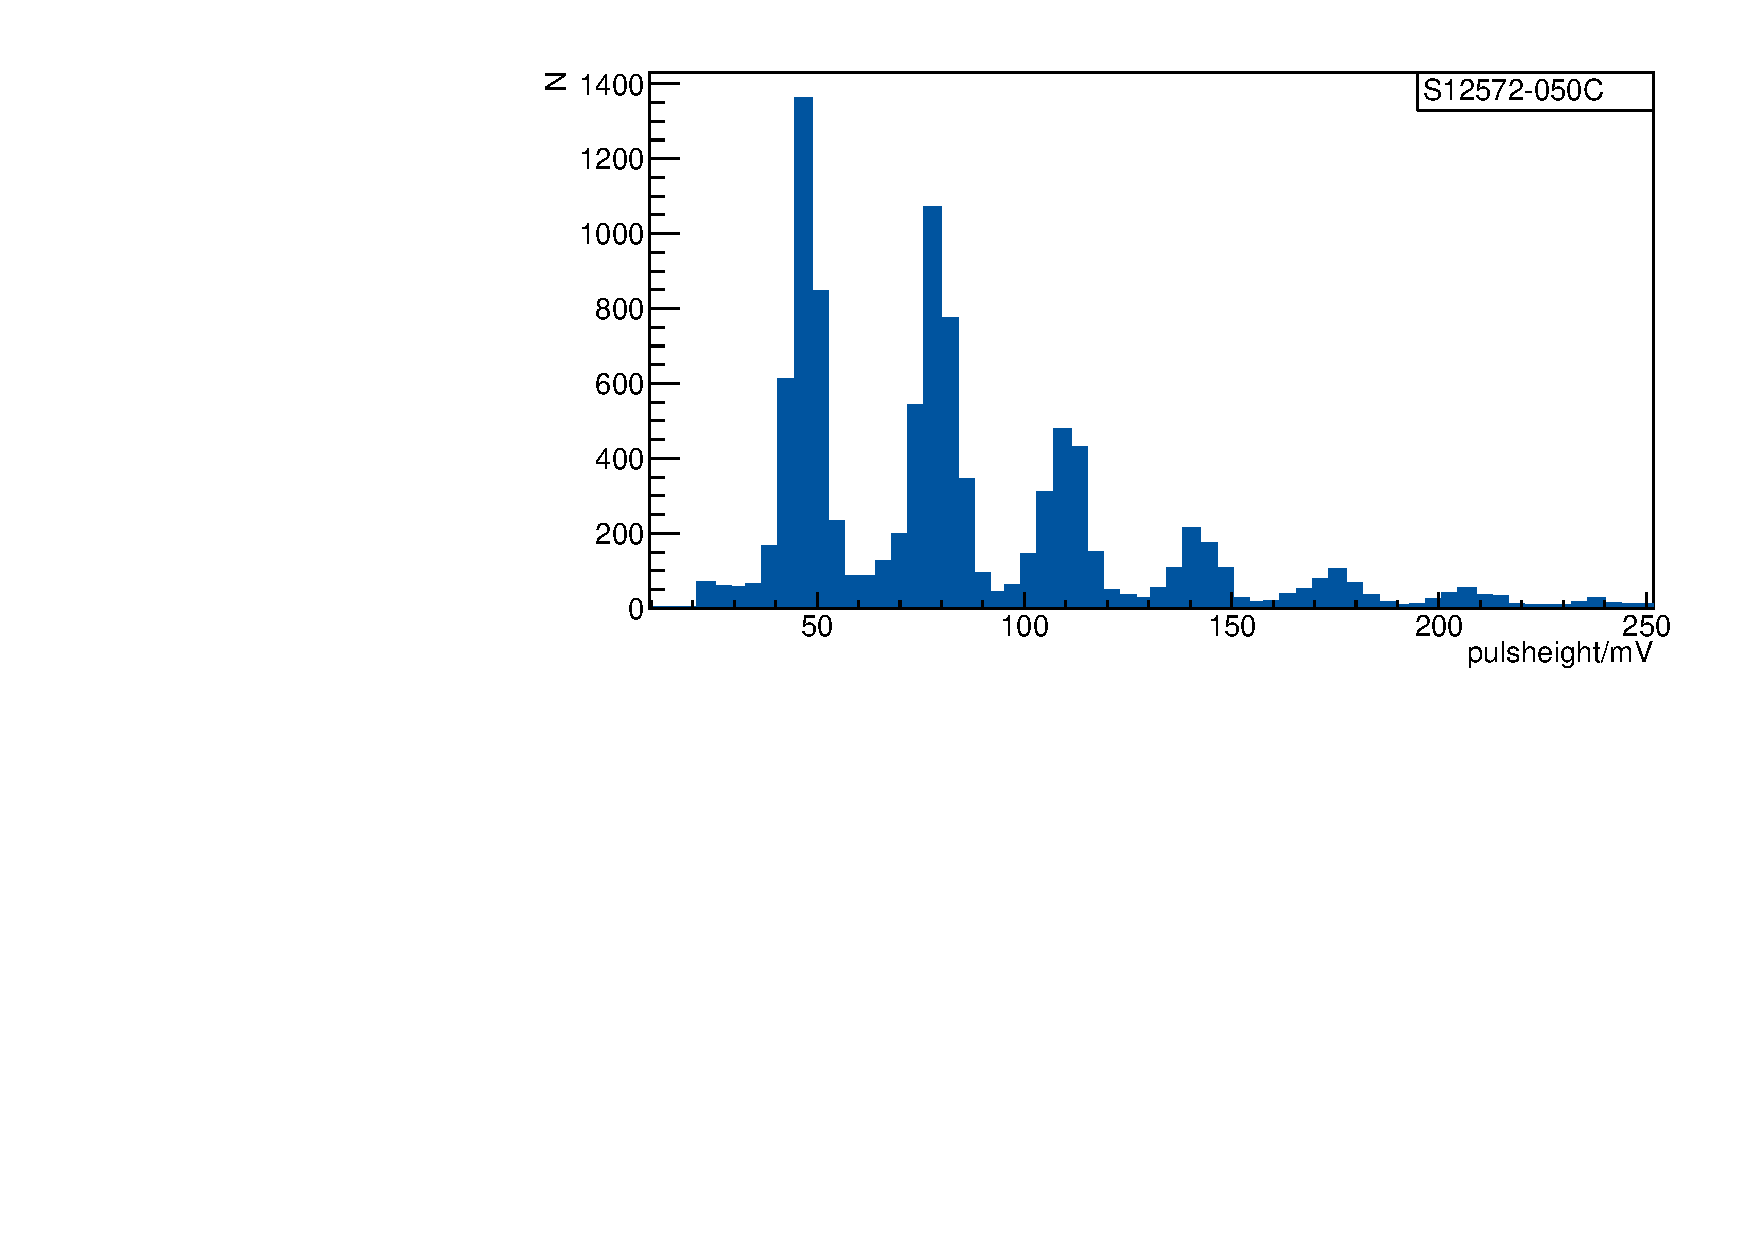
\includegraphics[width = .99\textwidth]{Figures/radermacher/S12572-050C.pdf}
	\end{minipage}
	\caption{fingerspectra for the testes SiPMs}
	\label{fingerspecs}
\end{figure}
\subsubsection{constant gain}
For the measurements with constant gain the value for the gain was assigned by using the given default voltage for $25\,\mathrm{^{\circ}C}$ while the cooling box was regulated to $25\,\mathrm{^{\circ}C}$. Afterwards the temperature was reduced in steps of 1 degree in a range between $25$ and $15\,\mathrm{^{\circ}C}$. Every step the gain was measure and controlled if it is the same as the default gain. Till this was reached the supplied voltage was regulated that one get the desired circumstances. Afterwards the noiserate was measured as shown in figure \ref{constGain_rate}.
As expected the noiserate increases with temperature due to thermally-generated carriers. Also one can see that the newer Hamamatsu product has significant higher noiserates.
\begin{figure}[h]
	\centering
	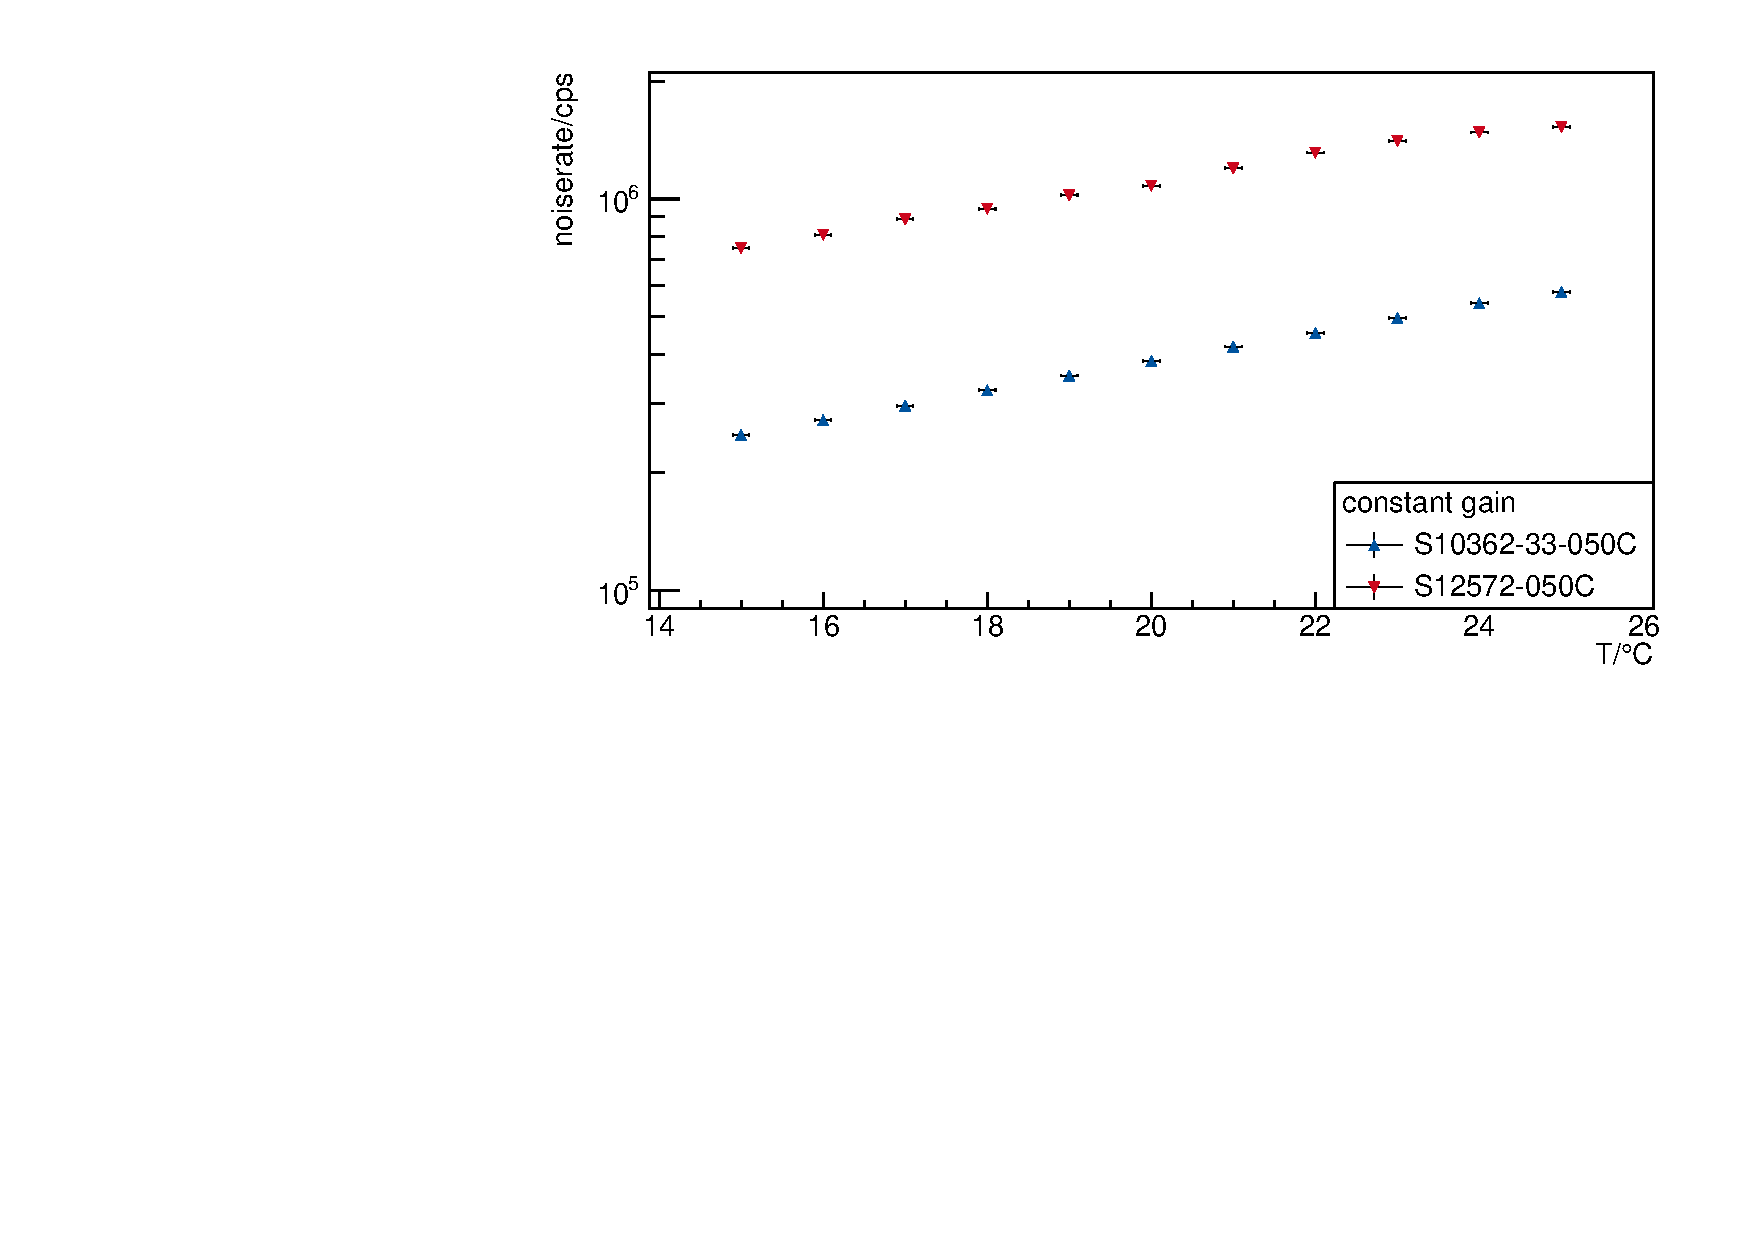
\includegraphics[width = 0.75 \textwidth]{Figures/radermacher/constGain_Rate.pdf}
	\caption{noiserate under temperature variation with constant gain}
	\label{constGain_rate}
\end{figure}
As a second result from this measurements it was possible to check the temperature regression coefficient. These values are given by Hamamatsu for every SiPM-Serie. For the S10362-33-050C the coefficient is predicted to $56\,\mathrm{mV/K}$, for the S12572-050C it is $60\,\mathrm{mV/K}$. Our measurements are in good agreement to this with $(56.6 \pm 0.5)\,\mathrm{mV/K}$ for S10362-33-050C and $(59.7 \pm 0.7)\,\mathrm{mV/K}$ for S12572-050C SiPMs. The results are shown in figure \ref{tempCoeff}. 
\begin{figure}[h]
	\centering
	\begin{minipage}[b]{0.49\textwidth}
		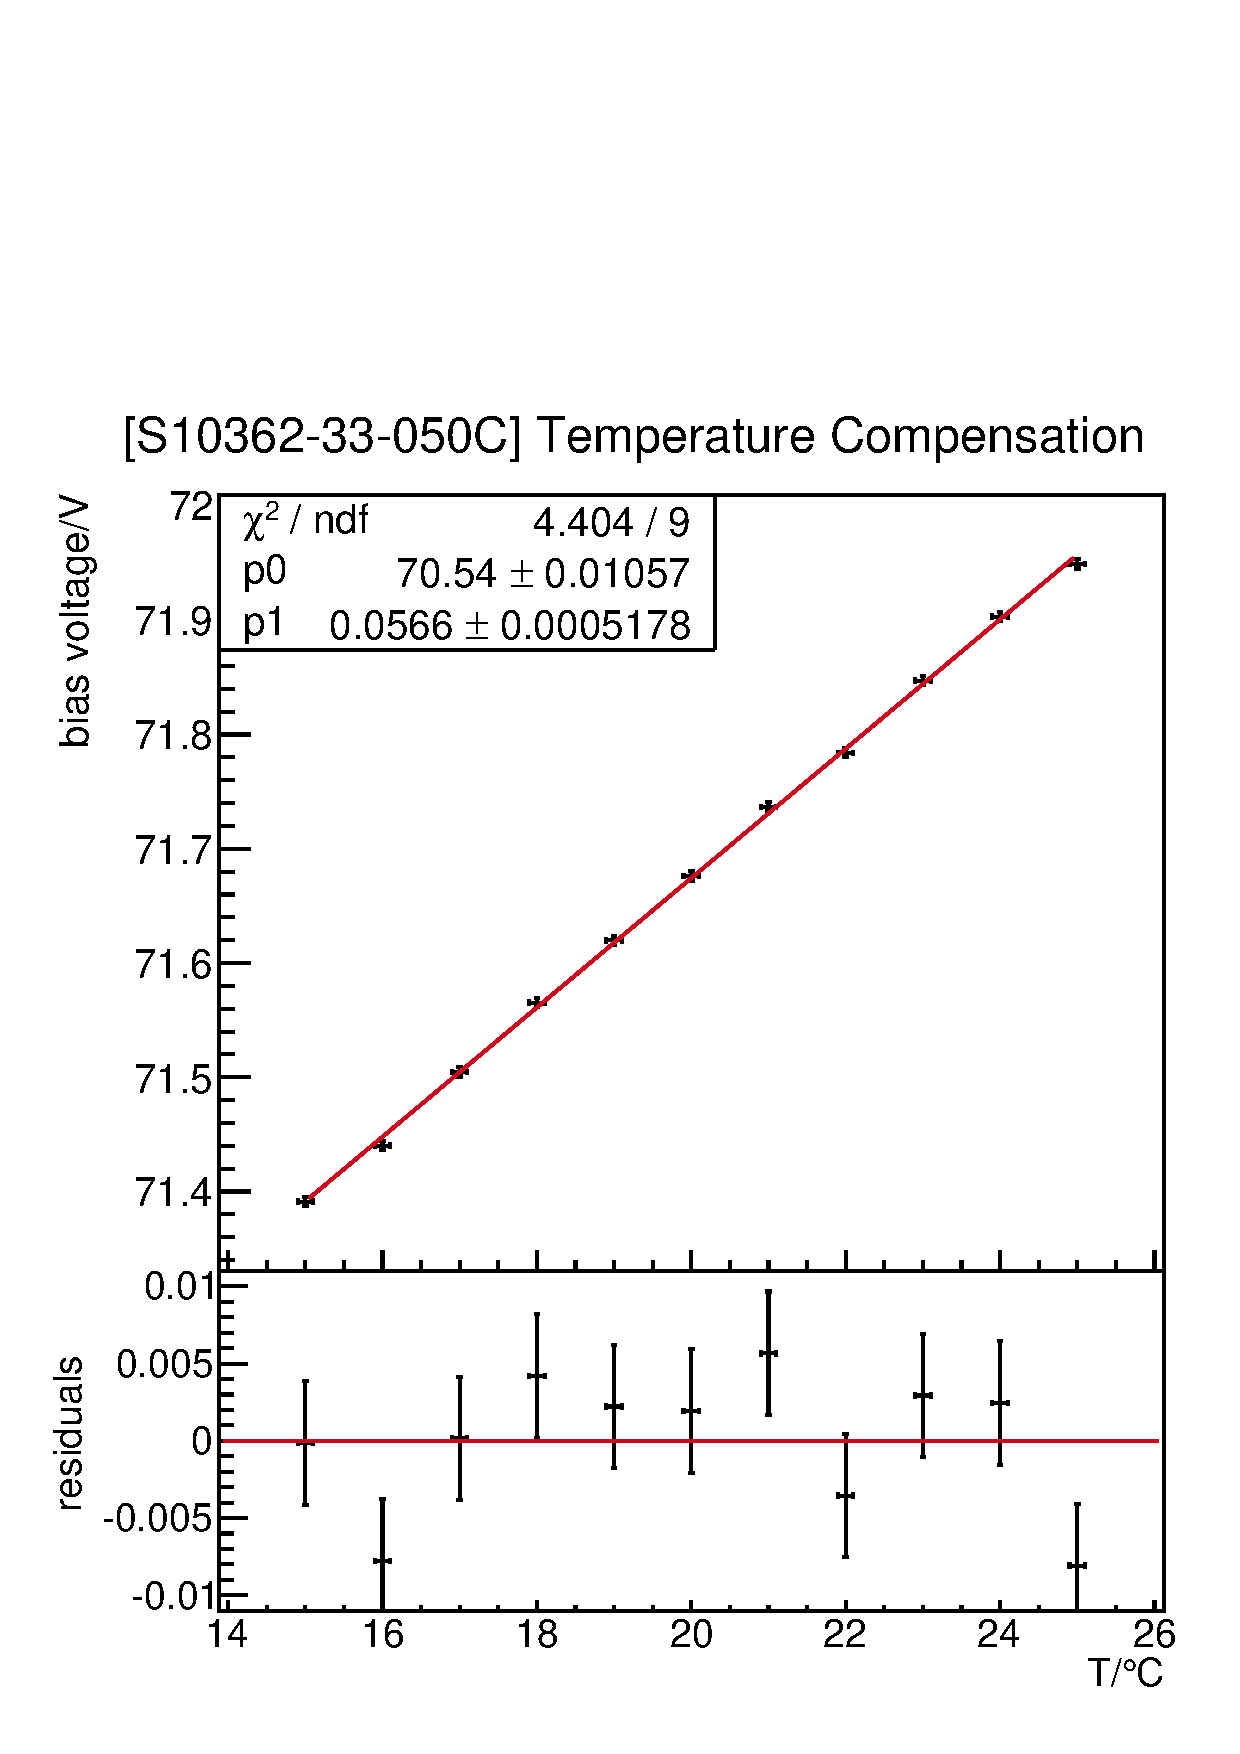
\includegraphics[width = 0.98\textwidth]{Figures/radermacher/TempReg_S10362.pdf}
	\end{minipage}	
	\begin{minipage}[b]{0.49\textwidth}
		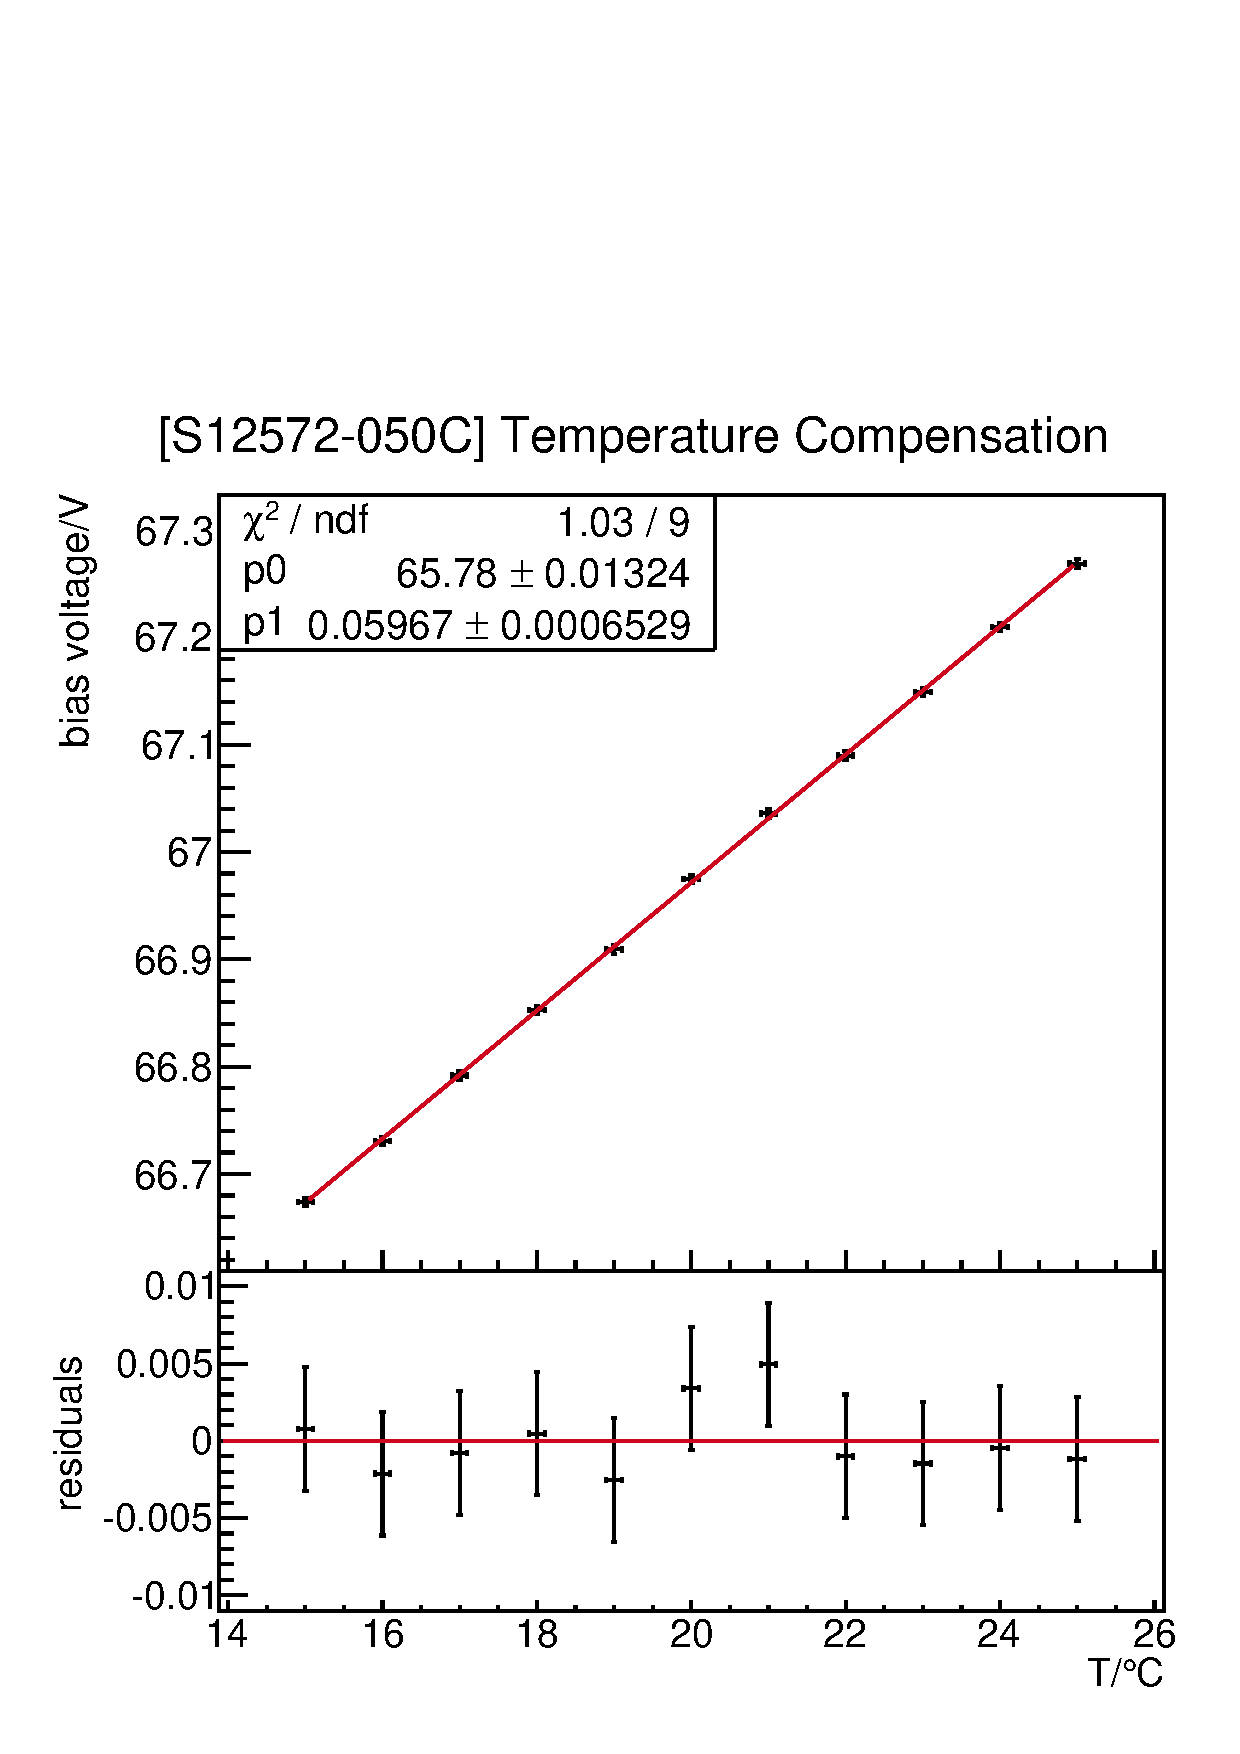
\includegraphics[width = 0.98\textwidth]{Figures/radermacher/TempReg_S12572.pdf}
	\end{minipage}
	\caption{Determination of the temperature progression coefficient}
	\label{tempCoeff}
\end{figure}

\subsubsection{constant bias voltage}
To measure the noiserate by keeping the bias voltage constant the voltage was set to the default voltage at $25\,\mathrm{^{\circ}C}$ and the temperature was regulated between $25$ and $15\,\mathrm{^{\circ}C}$ in steps of 1 degree. As shown in figure \ref{constVolt_rate} there is a linear increase with temperature. These increase is much higher for the newer Hamamatsu product S12572 with $39.4\,\mathrm{\%}$ as for the S10362-33-050C with $26.5\,\mathrm{\%}$ over a range of $10\,\mathrm{^{\circ}C}$. 
The gain otherwise shows a linear decrease with temperature due to the higher overvoltage on lower temperature as one can see in figure \ref{constVolt_gain}. The plateau by $15 - 17\,\mathrm{^{\circ}C}$ arised from smeared fingerspectra.  
\begin{figure}[h]
	\centering
	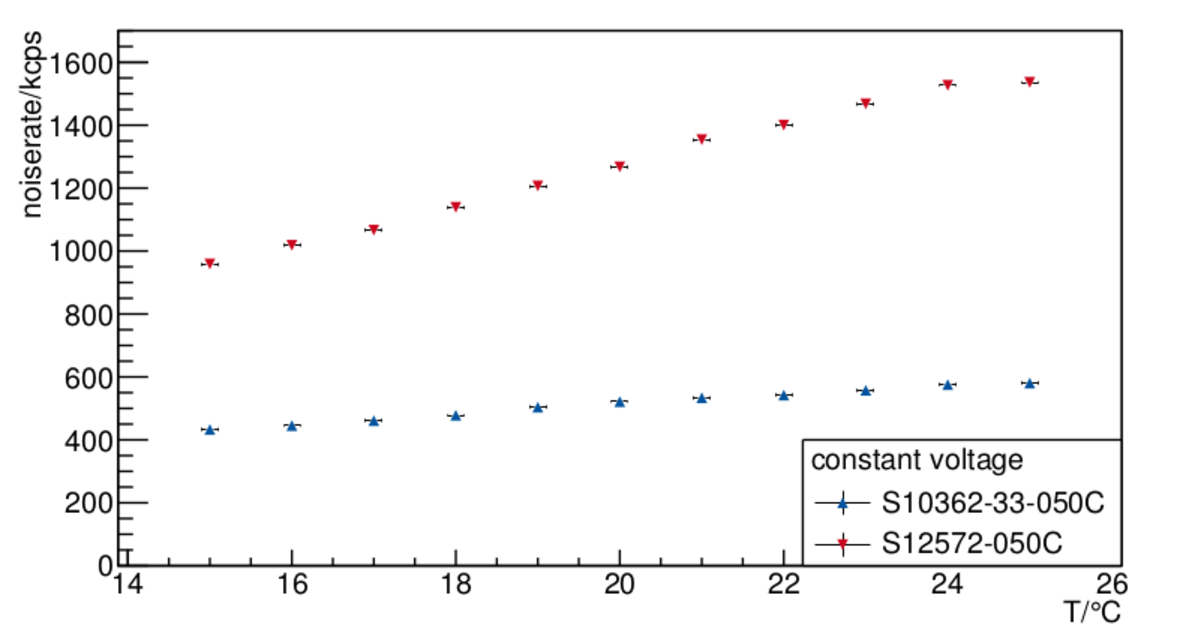
\includegraphics[width = 0.75 \textwidth]{Figures/radermacher/ConstVolt_Rate_linear.pdf}
	\caption{noiserate under temperature variation with constant bias voltage}
	\label{constVolt_rate}
\end{figure}
\begin{figure}[h]
	\centering
	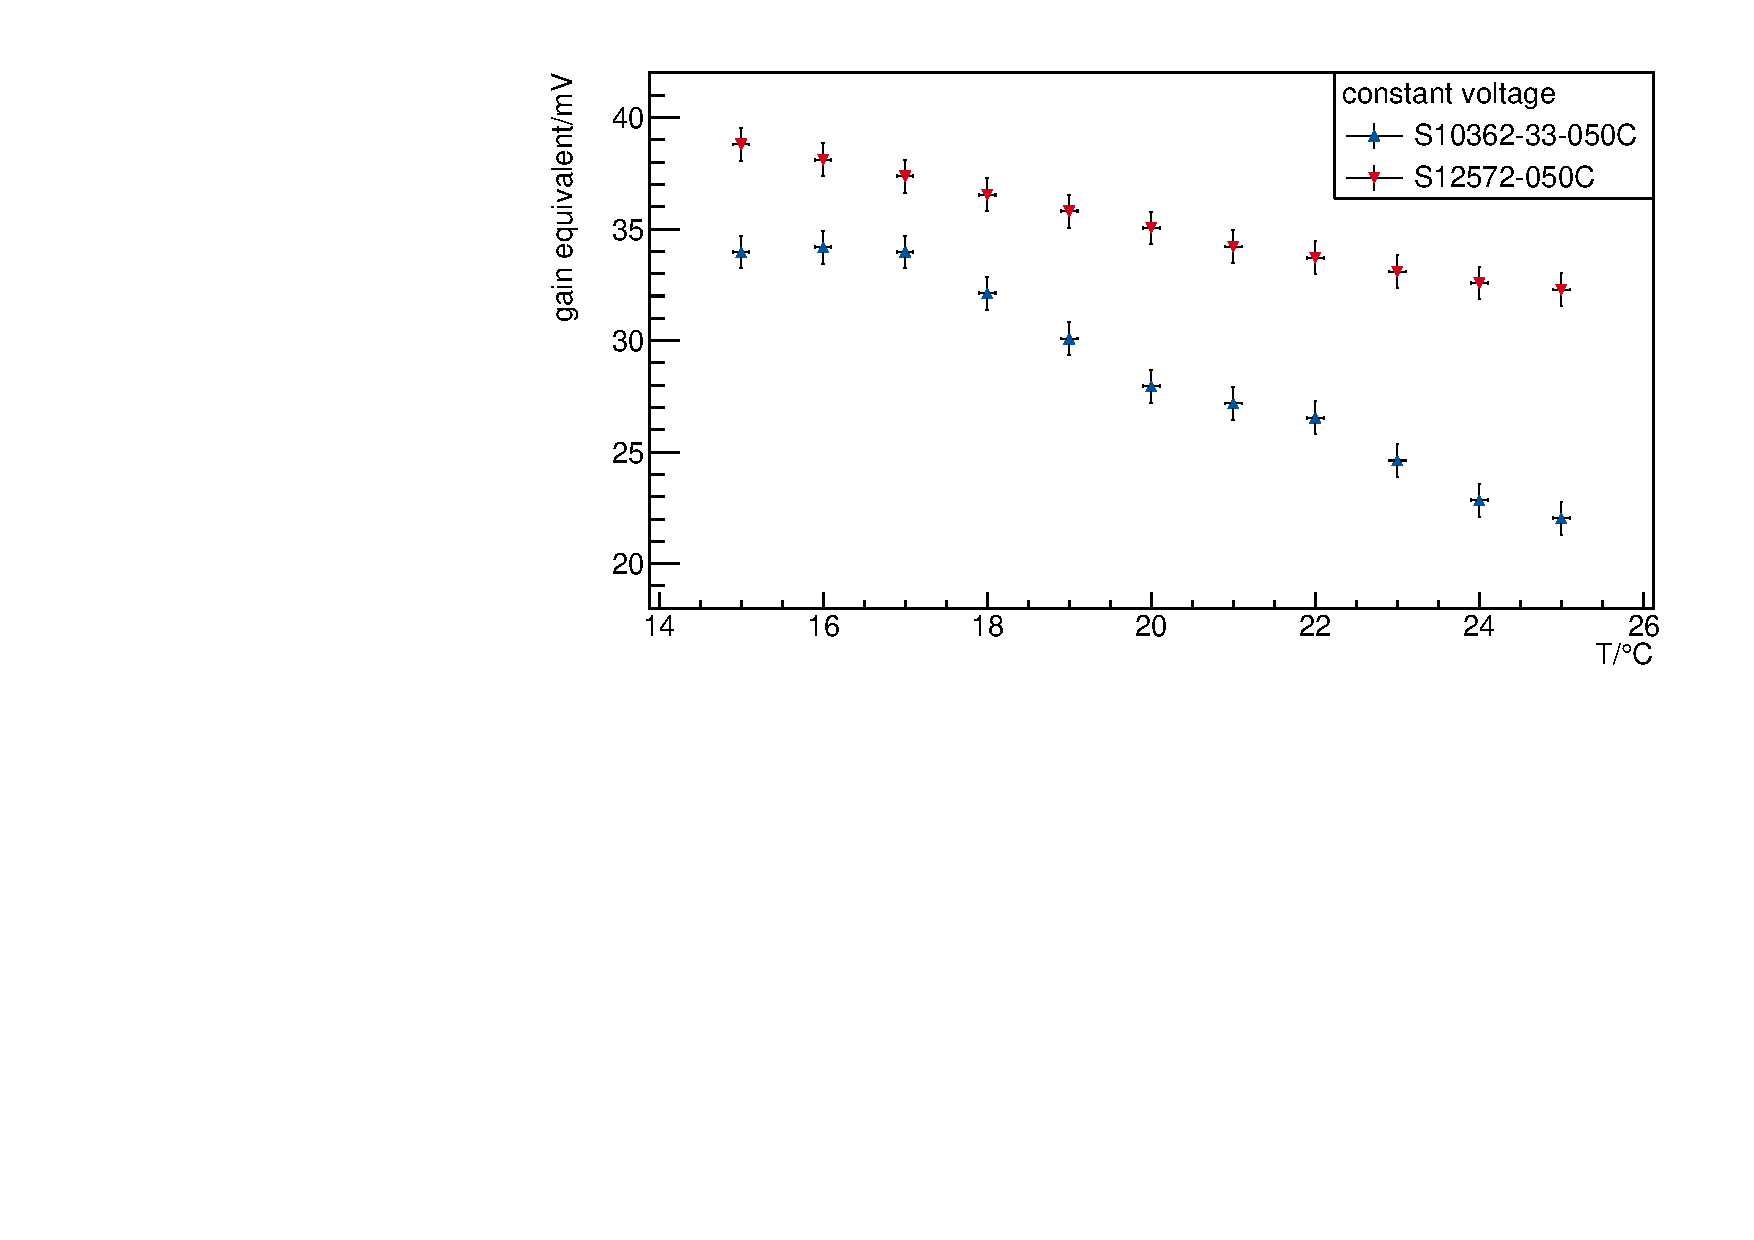
\includegraphics[width = 0.75 \textwidth]{Figures/radermacher/constVolt_Gain.pdf}
	\caption{Gain under temperature variation with constant bias voltage}
	\label{constVolt_gain}
\end{figure}
\subsubsection{constant temperature}
For measuring the noiserates with constant temperature this was set to $25\,\mathrm{^{\circ}C}$ and the bias voltage was raised in $50\,\mathrm{mV}$-steps. With more bias voltage the noiserate increase linear. Under these circumstances it is much higher for the S10362-33-050C with $62.8\,\mathrm{\%}$ instead of $16.0\,\mathrm{\%}$ for the S12572-050C over the range of $450\,\mathrm{mV}$ shown in figure \ref{constTemp_rate}. The trend of the gain as one can see in figure \ref{constTemp_gain} is not analytic but looks quite equal for both SiPMs.
\begin{figure}[h]
	\centering
	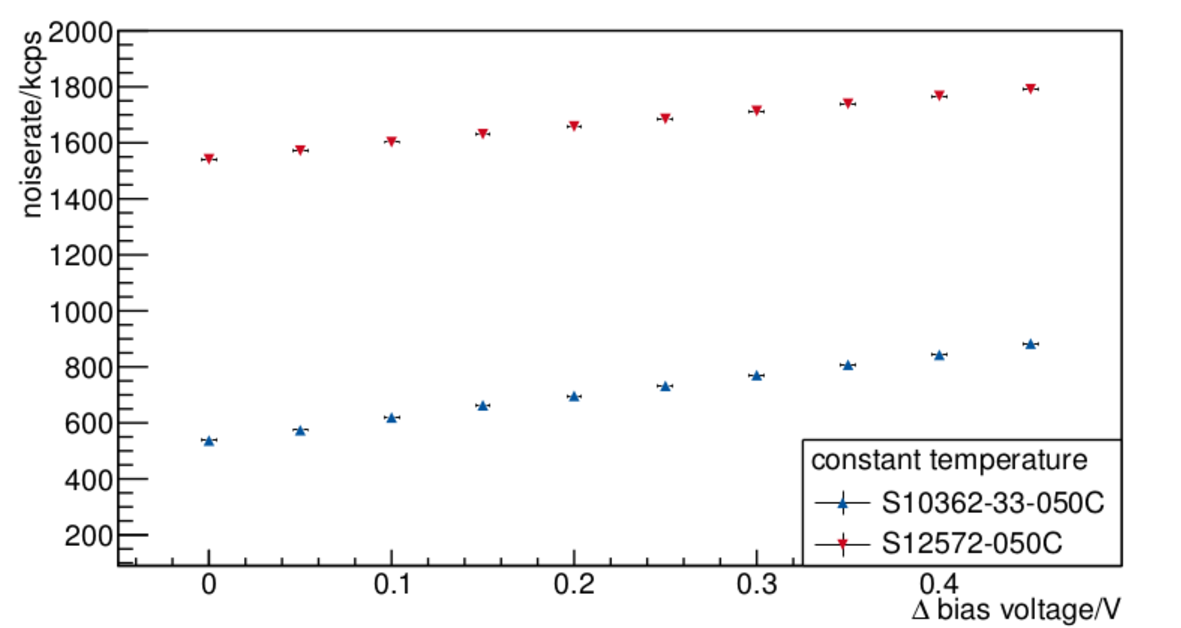
\includegraphics[width = 0.75 \textwidth]{Figures/radermacher/ConstTemp_Rate_linear.pdf}
	\caption{noiserate under variation of bias voltage with constant temperature}
	\label{constTemp_rate}
\end{figure}
\begin{figure}[h]
	\centering
	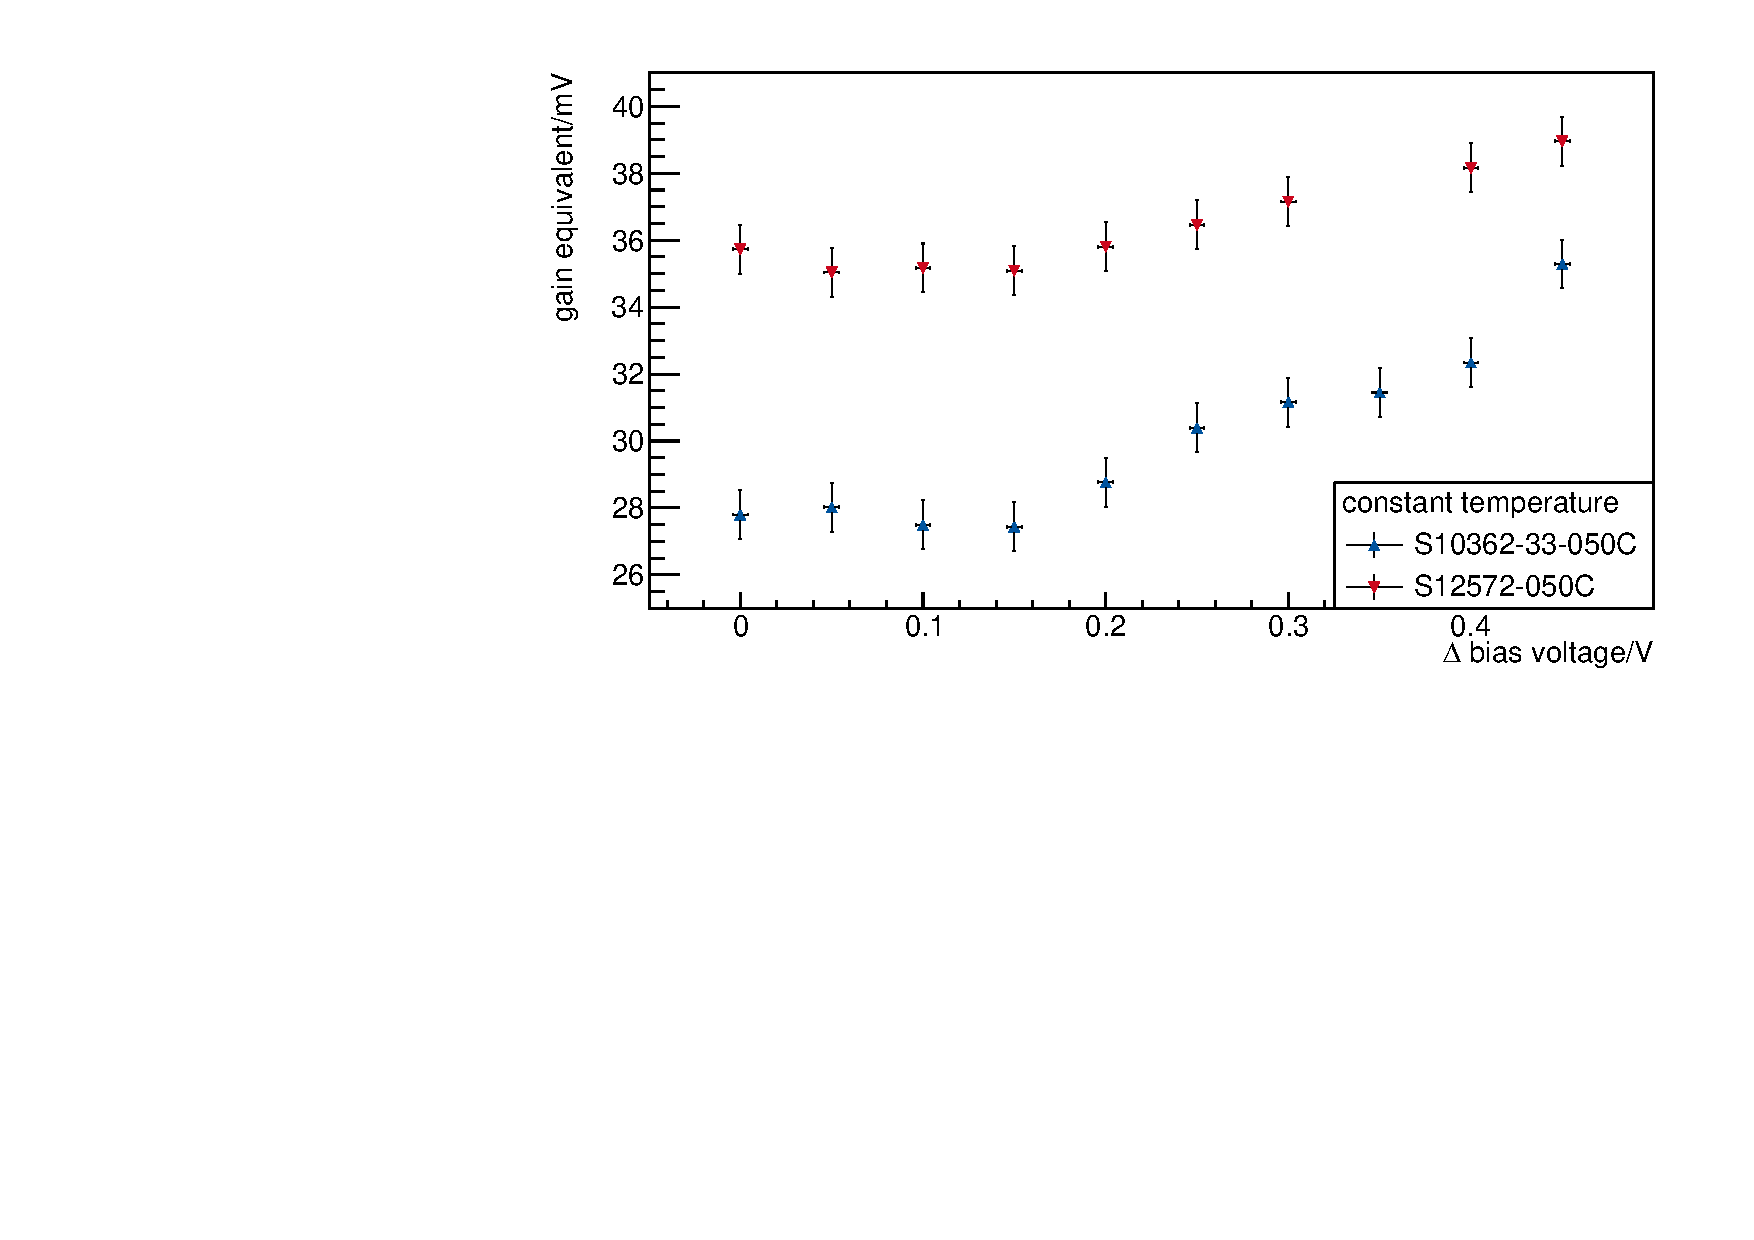
\includegraphics[width = 0.75 \textwidth]{Figures/radermacher/constTemp_Gain.pdf}
	\caption{Gain under variation of bias voltage with constant temperature}
	\label{constTemp_gain}
\end{figure}
\subsubsection{conclusion}
The measurements shown the expected behaviour on temperature variations. The temperature regression coefficient given by Hamamatsu has been certified and some quality criteria were studied. With help of this we choose to use the S10362-33-050C for our prototyp detectors until a newer SiPM-serie is presented because there are not enough improvements by using the S12572-050C due to clipping of the amplifier mentioned in chapter HIER KAPITEL UEBER NOISEPEAK EINFUEGEN. Therefore the higher gain is not needed and will maybe produce more signals in clipping. Unless a controlling of the bias voltage due to temperature change by counting in the asymmetry of the p.e. is done a better peaksresolution is not needed.
